\documentclass[11pt,runningheads,a4paper]{article}
\usepackage[utf8]{inputenc}
\usepackage{amsmath,amssymb,hyperref,array,xcolor,multicol,verbatim,mathpazo}
\usepackage[normalem]{ulem}
\usepackage[pdftex]{graphicx}
\usepackage{fullpage}
\usepackage{hyperref}
\usepackage{float}
\usepackage{listings}
%\usepackage{minted} %code highlighting, listings is bad for R
\usepackage{romannum}
\usepackage{enumitem} %description list
\newcommand{\DNA}[1]{\texttt{\uppercase{#1}}}
\begin{document}
%%%% In most cases you won't need to edit anything above this line %%%%
\title{{\LARGE Bioinformatics Supervision}\\
{\Large Michaelmas Term 2017}\\
{\Large --Problem Sheet 2--}}

\author{Supervisor: Sebastian Müller (Department of Plant Sciences)}
\date{}

\maketitle

Please hand in your work 24 hours prior to the supervision either to \texttt{sm934@cam.ac.uk} or at the Plant Sciences Department reception (make sure my name is on it).
Feel free to team up with other group members, the main aim is to understand the material.
If you hand in electronically, please name the file \texttt{group<x>\_<crsid>\_problemsheet<x>.<x>}

\begin{enumerate}
\section*{Phylogenetics}
  \item Considerable recent Bioinformatics research has focused on phylogenetics. What is the motivation for this work?
  \item Describe the differences in complexity and performance between parsimony and two distance phylogenetic methods. Also try to find another tree construction method not mentioned in the lecture and describe it conceptually.
    %	\item Describe with the aid of examples two different techniques for distance-based phylogeny. In each case discuss the issues of complexity and performance.
  \item Commonly used methods for traversing a binary tree include pre-order, in-order, and post-order.
    Suppose we need to implement the SmallParsimony algorithm using one of these traversal methods.
    Which one(s) would be suitable for our implementation? Explain your choice.
  \item  How is the score matrix used in phylogenetic tree building techniques? Hint: A prominent example is the PAM score matrix described on page 285 of Vol.\Romannum{1} (Compeau and Pevzner 2nd Edition).
  \item You are given the tree below with single-letter sequences at its leaves.
    Use the SmallParsimony algorithm to find the minimum parsimony cost for the given tree and identify the optimal state assignments for each node with $c(A; G) = 1$ and $c(A; A) = c(G; G) = 0$.
    \begin{figure}[h]
      \centering
      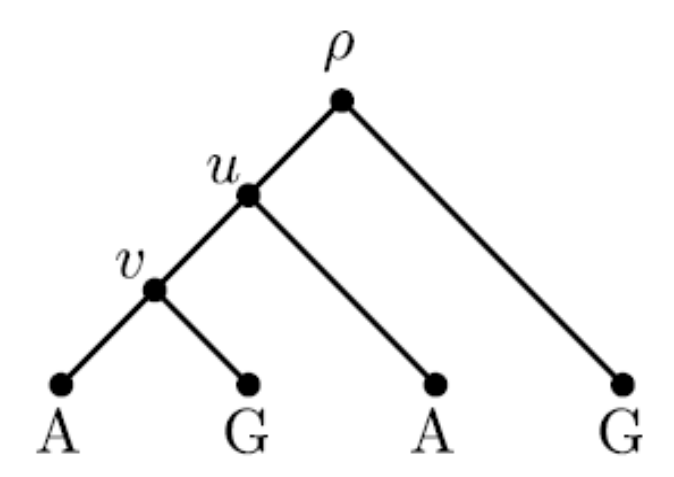
\includegraphics[scale=0.25]{img/Bioinformatics_Problem_Sheet2_fig1.png}
    \end{figure}
    %\begin{enumerate}
    %%Fitch and Sankkoff has been taken out of the lecture, Sankoff is now called Small Parsimony Problem
    %%\item Use the Fitch algorithm to find the minimum parsimony cost for the given tree and identify the optimal state assignments for each node, which have the minimum cost.
    %%\item Verify that we would also obtain the same minimum cost in part (a) by using the Sankoff algorithm with c(A; G) = 1 and c(A; A) = c(G; G) = 0.
    %%\item What are the optimal state assignments you would obtain from part (b)? Are there any discrepancies with those you found in part (a)? If there are, provide an explanation.
    %\end{enumerate}
  \item Given the following distance matrix, calculate an evolutionary tree using UPGMA:
  \nopagebreak
    \begin{table}[H]
      \centering
      \begin{tabular}{|l|r|r|r|l|l|l|}
        \hline
        & \multicolumn{1}{l|}{A} & \multicolumn{1}{l|}{B} & \multicolumn{1}{l|}{C} & D & E & F \\ \hline
        A & 0 & \multicolumn{1}{l|}{} & \multicolumn{1}{l|}{} &  &  &  \\ \hline
        B & 2 & 0 & \multicolumn{1}{l|}{} &  &  &  \\ \hline
        C & 4 & 4 & 0 &  &  &  \\ \hline
        D & 6 & 6 & 6 & \multicolumn{1}{r|}{0} &  &  \\ \hline
        E & 6 & 6 & 6 & \multicolumn{1}{r|}{4} & \multicolumn{1}{r|}{0} &  \\ \hline
        F & 8 & 8 & 8 & \multicolumn{1}{r|}{8} & \multicolumn{1}{r|}{8} & \multicolumn{1}{r|}{0} \\ \hline
      \end{tabular}
      \label{}
    \end{table}
  \item  Given the following distance matrix, calculate an evolutionary tree using Neighbour-Joining algorithm:
  \nopagebreak
    \begin{table}[H]
      \centering
      \begin{tabular}{|l|r|r|r|l|l|}
        \hline
        & \multicolumn{1}{l|}{A} & \multicolumn{1}{l|}{B} & \multicolumn{1}{l|}{C} & D & E \\ \hline
        A & 0 & \multicolumn{1}{l|}{} & \multicolumn{1}{l|}{} &  &  \\ \hline
        B & 5 & 0 & \multicolumn{1}{l|}{} &  &  \\ \hline
        C & 4 & 7 & 0 &  &  \\ \hline
        D & 7 & 10 & 7 & \multicolumn{1}{r|}{0} &  \\ \hline
        E & 6 & 9 & 6 & \multicolumn{1}{r|}{5} & \multicolumn{1}{r|}{0} \\ \hline
      \end{tabular}
      \label{}
    \end{table}

\section*{Pattern Matching}\label{sec:burrows_wheeler_transformation}
\item  Implement \textit{TRIE(patterns)} in a language of your choice using the patterns given in the book (Compeau, 2nd Edition, Vol II, page 124) 

\textit{patterns} =  ``ananas'', ``and", ``antenna", ``banana", ``bandana", ``nab", ``nana", ``pan"

\item Implement a function \textit{PrefixTrieMatching(Text, Trie)} which checks whether any string from $Patterns$ matches a prefix of the string $Text$ = "panamabananas" (see page 125). Also try with $Text$ = ``namabananas".

  \item Discuss the main features of the Burrows-Wheeler transform (BWT) using the following example: T = \DNA{GATATCA}\$. Also, explain the reversibility of BWT.

\item  \textbf{OPTIONAL}  Implement \textit{TrieMatching(Text,Trie)} to allow pattern matching also within $Text$ as opposed to only the prefix.

\end{enumerate}
    \end{document}
